\section{Taylor Polynomials}\label{sec:taylorpolynomials}

Consider a function $y=f(x)$ and a point $\big(c,f(c)\big)$. The derivative, $f'(c)$, gives the instantaneous rate of change of $f$ at $x=c$. Of all lines that pass through the point $\big(c,f(c)\big)$, the line that best approximates $f$ at this point is the tangent line; that is, the line whose slope (rate of change) is $f'(c)$.

In Figure \ref{fig:taypolyintroa}, we see a function $y=f(x)$ graphed. The table below the graph shows that $f(0)=2$ and $\fp(0) = 1$; therefore, the tangent line to $f$ at $x=0$ is $p_1(x) = 1(x-0)+2 = x+2$. The tangent line is also given in the figure. Note that ``near'' $x=0$, $p_1(x) \approx f(x)$; that is, the tangent line approximates $f$ well.

\mtable{.78}{Plotting $y=f(x)$ and a table of derivatives of $f$ evaluated at 0.}{fig:taypolyintroa}{%
\begin{tabular}{m{.6\textwidth} m{.3\textwidth}}
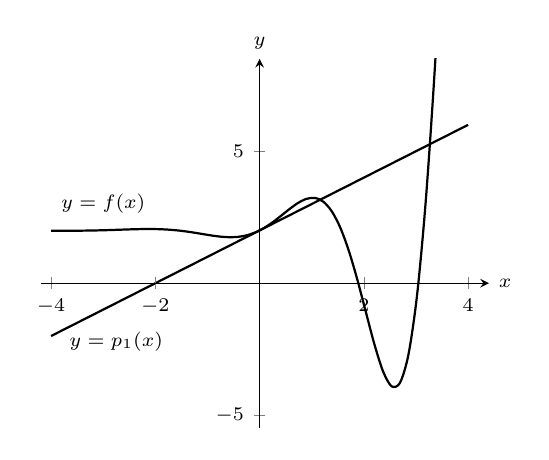
\begin{tikzpicture}
\begin{axis}[width=.6\textwidth,%
tick label style={font=\scriptsize},axis y line=middle,axis x line=middle,name=myplot,axis on top,%
%			xtick={2,4,6,8,10},% 
%			extra x ticks={3.14,1.57},
%			extra x tick labels={$\pi$,$\pi/2$},
%			ytick={-1,-2,1,2},
			%minor y tick num=1,%extra y ticks={-5,-3,...,7},%
%			minor x tick num=4,
			ymin=-5.5,ymax=8.5,%
			xmin=-4.2,xmax=4.4%
]

\addplot [{\colorone},domain=-4:4,smooth,thick,samples=50] {exp(x)*sin(deg(x))*cos(deg(x))+2};
\addplot [{\colortwo},domain=-4:4,thick] {x+2};

\draw (axis cs:-3.,3) node {\scriptsize $y=f(x)$};
\draw (axis cs:-2.75,-2.2) node {\scriptsize $y=p_1(x)$};

\end{axis}

\node [right] at (myplot.right of origin) {\scriptsize $x$};
\node [above] at (myplot.above origin) {\scriptsize $y$};

\end{tikzpicture} &
\begin{tabular}{l}
$f(0) = 2$ \\ [2mm] 
$\fp(0) = 1$ \\ [2mm] 	
$\fpp(0) = 2$ \\ [2mm]
$\fp''(0) = -1$\\ [2mm]
$f\,^{(4)}(0)=-12$ \\ [2mm]
 $f\,^{(5)}(0)=-19$
\end{tabular} 
\end{tabular}
}

One shortcoming of this approximation is that the tangent line only matches the slope of $f$; it does not, for instance, match the concavity of $f$. We can find a polynomial, $p_2(x)$, that does match the concavity without much difficulty, though. The table in Figure \ref{fig:taypolyintroa} gives the following information:
$$f(0) = 2 \qquad \fp(0) = 1\qquad \fp'(0) = 2.$$
Therefore, we want our polynomial $p_2(x)$ to have these same properties. That is, we need $$p_2(0) = 2 \qquad p_2'(0) = 1 \qquad p_2''(0) = 2.$$

This is simply an initial--value problem.  To keep $p_2(x)$ as simple as possible, we'll assume that not only  $p_2''(0)=2$, but that $p_2''(x)=2$. That is, the second derivative of $p_2$ is  constant.

If $p_2''(x) = 2$, then $p_2'(x) = 2x+C$ for some constant $C$. Since we have determined that $p_2'(0) = 1$, we find that $C=1$ and so $p_2'(x) = 2x+1$. Finally, we can compute $p_2(x) = x^2+x+C$. Using our initial values, we know $p_2(0) = 2$ so $C=2.$ We conclude that $p_2(x) = x^2+x+2.$ This function is plotted with $f$ in Figure \ref{fig:taypolyintrobc}.



\begin{figure}
	\begin{subfigure}[t]{0.5\textwidth}
	\begin{tikzpicture}
		\begin{axis}[ %width=\linewidth,%
		tick label style={font=\scriptsize},axis y line=middle,axis x line=middle,name=myplot,axis on top,%
		%			xtick={2,4,6,8,10},% 
		%			extra x ticks={3.14,1.57},
		%			extra x tick labels={$\pi$,$\pi/2$},
		%			ytick={-1,-2,1,2},
					%minor y tick num=1,%extra y ticks={-5,-3,...,7},%
		%			minor x tick num=4,
					ymin=-5.5,ymax=8.5,%
					xmin=-4.2,xmax=4.4%
		]
		
		\addplot [{\colorone},domain=-4:4,smooth,thick,samples=50] {exp(x)*sin(deg(x))*cos(deg(x))+2};
		\addplot [{\colortwo},domain=-4:4,thick,smooth] {x^2+x+2};
		\addplot [{\colortwo!40},domain=-4:4,thick,smooth] {-x^4/2-x^3/6+x^2+x+2};
		
		\draw (axis cs:-3.,3.5) node {\scriptsize $y=p_2(x)$};
		\draw (axis cs:-3.1,-2.5) node {\scriptsize $y=p_4(x)$};
		
		\end{axis}
		
		\node [right] at (myplot.right of origin) {\scriptsize $x$};
		\node [above] at (myplot.above origin) {\scriptsize $y$};
		
		\end{tikzpicture}
        \label{fig:taypolyintrob}
        \caption{Plotting $f$, $p_2$ and $p_4$.} 
    \end{subfigure}% 
    \begin{subfigure}[t]{0.5\textwidth}
    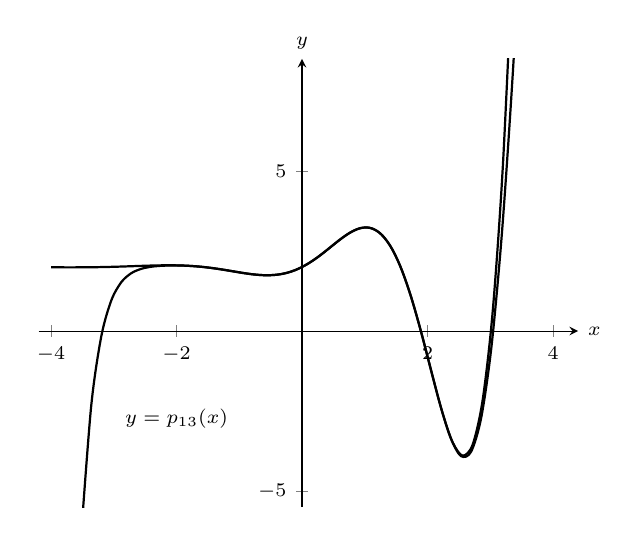
\begin{tikzpicture}
    \begin{axis}[ %width=.5\textwidth,%
    tick label style={font=\scriptsize},axis y line=middle,axis x line=middle,name=myplot,axis on top,%
    %			xtick={2,4,6,8,10},% 
    %			extra x ticks={3.14,1.57},
    %			extra x tick labels={$\pi$,$\pi/2$},
    %			ytick={-1,-2,1,2},
    			%minor y tick num=1,%extra y ticks={-5,-3,...,7},%
    %			minor x tick num=4,
    			ymin=-5.5,ymax=8.5,%
    			xmin=-4.2,xmax=4.4%
    ]
    
    \addplot [{\colorone},domain=-4:4,smooth,thick,samples=50] {exp(x)*sin(deg(x))*cos(deg(x))+2};
    \addplot [{\colortwo},domain=-4:4,thick,smooth] coordinates {(-3.52,-6.364)(-3.36,-2.334)(-3.2,-0.1706)(-3.04,0.9569)(-2.88,1.528)(-2.72,1.809)(-2.56,1.944)(-2.4,2.009)(-2.24,2.038)(-2.08,2.048)(-1.92,2.046)(-1.76,2.031)(-1.6,2.006)(-1.44,1.969)(-1.28,1.924)(-1.12,1.872)(-0.96,1.82)(-0.8,1.775)(-0.64,1.747)(-0.48,1.747)(-0.32,1.783)(-0.16,1.866)(0,2.)(0.16,2.185)(0.32,2.411)(0.48,2.662)(0.64,2.908)(0.8,3.112)(0.96,3.227)(1.12,3.202)(1.28,2.988)(1.44,2.546)(1.6,1.855)(1.76,0.9264)(1.92,-0.1926)(2.08,-1.406)(2.24,-2.565)(2.4,-3.474)(2.56,-3.891)(2.72,-3.542)(2.88,-2.133)(3.04,0.6461)(3.2,5.139)(3.36,11.79)};
    %\addplot [{\colortwo!40},domain=-4:4,thick,smooth] {-x^4/2-x^3/6+x^2+x+2};
    
    %\draw (axis cs:-3.,3.5) node {\scriptsize $y=p_2(x)$};
    \draw (axis cs:-2,-2.75) node {\scriptsize $y=p_{13}(x)$};
    
    \end{axis}
    
    \node [right] at (myplot.right of origin) {\scriptsize $x$};
    \node [above] at (myplot.above origin) {\scriptsize $y$};
    
    \end{tikzpicture}
        \label{fig:taypolyintroc}
        \caption{Plotting $f$ and $p_{13}$.}    
    \end{subfigure} 
    \caption{ \label{fig:taypolyintrobc}}
\end{figure}






We can repeat this approximation process by creating polynomials of higher degree that match more of the derivatives of $f$ at $x=0$. In general, a polynomial of degree $n$ can be created to match the first $n$ derivatives of $f$. Figure \ref{fig:taypolyintrob} also shows $p_4(x)= -x^4/2-x^3/6+x^2+x+2$, whose first four derivatives at 0 match those of $f$. (Using the table in Figure \ref{fig:taypolyintroa}, start with $p_4^{(4)}(x)=-12$ and solve the related initial--value problem.)

As we use more and more derivatives, our polynomial approximation to $f$ gets better and better. In this example, the interval on which the approximation is ``good'' gets bigger and bigger. Figure \ref{fig:taypolyintroc} shows $p_{13}(x)$; we can visually affirm that this polynomial approximates $f$ very well on $[-2,3]$. (The polynomial $p_{13}(x)$ is not particularly ``nice''. It is {\scriptsize $$ \frac{16901x^{13}}{6227020800}+\frac{13x^{12}}{1209600}-\frac{1321x^{11}}{39916800}-\frac{779x^{10}}{1814400}-\frac{359x^9}{362880}+\frac{x^8}{240}+\frac{139x^7}{5040}+\frac{11 x^6}{360}-\frac{19x^5}{120}-\frac{x^4}{2}-\frac{x^3}{6}+x^2+x+2.)$$}

The polynomials we have created are examples of \emph{Taylor polynomials}, named after the British mathematician Brook Taylor who made important discoveries about such functions. While we created the above Taylor polynomials by solving initial--value problems, it can be shown that Taylor polynomials follow a general pattern that make their formation much more direct. This is described in the following definition.


\begin{definition}{Taylor Polynomial, Maclaurin Polynomial}{def:taypoly}
{Let $f$ be a function whose first $n$ derivatives exist at $x=c$.
\index{Taylor Polynomial!definition}\index{Maclaurin Polynomial!definition} \index{Maclaurin Polynomial|see{Taylor Polynomial}}
\begin{enumerate}
\item		The \textbf{Taylor polynomial of degree $n$ of $f$ at $x=c$} is 
				{$$p_n(x) = f(c) + \fp(c)(x-c) + \frac{\fpp(c)}{2!}(x-c)^2+\frac{\fp''(c)}{3!}(x-c)^3+\cdots+\frac{f\,^{(n)}(c)}{n!}(x-c)^n.$$}

\item		A special case of the Taylor polynomial is the Maclaurin polynomial, where $c=0$. That is, the \textbf{Maclaurin polynomial of degree $n$ of $f$} is 
{$$p_n(x) = f(0) + \fp(0)x + \frac{\fpp(0)}{2!}x^2+\frac{\fp''(0)}{3!}x^3+\cdots+\frac{f\,^{(n)}(0)}{n!}x^n.$$}

\end{enumerate}
}
\end{definition}


We will practice creating Taylor and Maclaurin polynomials in the following examples.\\


\begin{example}{Finding and using Maclaurin polynomials}{ex_taypoly1}{
\begin{enumerate}
\item		Find the $n^\text{th}$ Maclaurin polynomial for $f(x) = e^x$.
\item		Use $p_5(x)$ to approximate the value of $e$.
\end{enumerate}
}
\end{example}


\begin{solution}
{\begin{enumerate}
\item We start with creating a table of the derivatives of $e^x$ evaluated at $x=0$. In this particular case, this is relatively simple, as shown in Table \ref{fig:taypoly1a}.


\mTable{.4}{The derivatives of $f(x)=e^x$ evaluated at $x=0$.}{fig:taypoly1a}{%
\begin{tabular}{lll}
$f(x) = e^x $&$\Rightarrow $&$f(0) = 1$\\
$\fp(x) = e^x $&$\Rightarrow $&$\fp(0) = 1$\\
$\fp'(x) = e^x $&$\Rightarrow $&$\fp'(0) = 1$\\
$\ \vdots $& &$\ \vdots$\\
$f\,^{(n)}(x) = e^x $&$\Rightarrow $&$f\,^{(n)}(0) = 1$
\end{tabular}
}
By the definition of the Maclaurin polynomial, we have 

\begin{align*}
p_n(x) &= f(0) + \fp(0)x + \frac{\fpp(0)}{2!}x^2+\frac{\fp''(0)}{3!}x^3+\cdots+\frac{f\,^n(0)}{n!}x^n\\
			&= 1+x+\frac{1}{2}x^2+\frac{1}{6}x^3 + \frac{1}{24}x^4 + \cdots + \frac{1}{n!}x^n.
\end{align*}

\item	Using our answer from part 1, we have $$p_5 = 1+x+\frac{1}{2}x^2+\frac{1}{6}x^3 + \frac{1}{24}x^4 + \frac{1}{120}x^5.$$ To approximate the value of $e$, note that $e = e^1 = f(1) \approx p_5(1).$ It is very straightforward to evaluate $p_5(1)$:
$$p_5(1) = 1+1+\frac12+\frac16+\frac1{24}+\frac1{120} = \frac{163}{60} \approx 2.71667.$$

A plot of $f(x)=e^x$ and $p_5(x)$ is given in Figure \ref{fig:taypoly1b}.

\mfigure{.8}{A plot of $f(x)=e^x$ and its 5$^\text{th}$ degree Maclaurin polynomial $p_5(x)$.}{fig:taypoly1b}{ %
\begin{tikzpicture}
\begin{axis}[ %width=\marginparwidth+25pt,%
tick label style={font=\scriptsize},axis y line=middle,axis x line=middle,name=myplot,axis on top,%
%			xtick={2,4,6,8,10},% 
%			extra x ticks={3.14,1.57},
%			extra x tick labels={$\pi$,$\pi/2$},
%			ytick={-1,-2,1,2},
			%minor y tick num=1,%extra y ticks={-5,-3,...,7},%
%			minor x tick num=4,
			ymin=-3,ymax=11,%
			xmin=-3.75,xmax=2.9%
]

\addplot [{\colorone},domain=-3.5:2.5,smooth,thick,samples=50] {exp(x)};
\addplot [{\colortwo},domain=-4:4,smooth,thick] coordinates {(-3.5,-1.645)(-3.39,-1.365)(-3.28,-1.123)(-3.17,-0.9148)(-3.06,-0.7362)(-3.,-0.65)(-2.89,-0.5103)(-2.78,-0.3917)(-2.67,-0.2911)(-2.56,-0.
2061)(-2.45,-0.1341)(-2.34,-0.07308)(-2.23,-0.02097)(-2.12,0.02397)(-
2.01,0.06332)(-1.9,0.0985)(-1.79,0.1308)(-1.68,0.1613)(-1.57,0.1911)(-
1.46,0.2212)(-1.35,0.2522)(-1.24,0.2851)(-1.13,0.3205)(-1.02,0.3592)(-
0.91,0.4018)(-0.8,0.449)(-0.69,0.5014)(-0.58,0.5598)(-0.47,0.625)(-0.
36,0.6977)(-0.25,0.7788)(-0.14,0.8694)(-0.03,0.9704)(0.08,1.083)(0.19,
1.209)(0.3,1.35)(0.41,1.507)(0.52,1.682)(0.63,1.878)(0.74,2.096)(0.85,
2.339)(0.96,2.61)(1.07,2.913)(1.18,3.25)(1.29,3.625)(1.4,4.042)(1.51,
4.506)(1.62,5.021)(1.73,5.592)(1.84,6.224)(1.95,6.924)(2.06,7.698)(2.
17,8.552)(2.28,9.494)(2.39,10.53)(2.5,11.67)};
%\addplot [{\colortwo!40},domain=-4:4,thick,smooth] {-x^4/2-x^3/6+x^2+x+2};

\draw (axis cs:-3.,-2) node {\scriptsize $y=p_5(x)$};
%\draw (axis cs:-2,-2.75) node {\scriptsize $y=p_{13}(x)$};

\end{axis}

\node [right] at (myplot.right of origin) {\scriptsize $x$};
\node [above] at (myplot.above origin) {\scriptsize $y$};

\end{tikzpicture} %
}
\end{enumerate}
}
\end{solution}


\begin{example}{Finding and using Taylor polynomials}{ex_taypoly2}{
\begin{enumerate}
\item		Find the $n^\text{th}$ Taylor polynomial of $y=\ln x$ at $x=1$.
\item		Use $p_6(x)$ to approximate the value of $\ln 1.5$.
\item		Use $p_6(x)$ to approximate the value of $\ln 2$. 
\end{enumerate}
}
\end{example}


\begin{solution}
{\begin{enumerate}
\item		We begin by creating a table of derivatives of $\ln x$ evaluated at $x=1$. While this is not as straightforward as it was in the previous example, a pattern does emerge, as shown in Table \ref{fig:taypoly2a}.
\mTable{.5}{Derivatives of $\ln x$ evaluated at $x=1$.}{fig:taypoly2a}{%
\begin{tabular}{lll}
$f(x) = \ln x $&$\Rightarrow $&$f(1) = 0$\\
$\fp(x) = 1/x $&$\Rightarrow $&$\fp(1) = 1$\\
$\fp'(x) = -1/x^2 $&$\Rightarrow $&$\fp'(1) = -1$\\
$\fp''(x) = 2/x^3 $&$\Rightarrow $&$\fp''(1) = 2$\\
$f\,^{(4)}(x) = -6/x^4 $&$\Rightarrow $&$f\,^{(4)}(1) = -6$\\
$\ \vdots $& &$\ \vdots$\\
$f\,^{(n)}(x) = $ &$\Rightarrow$ & $f\,^{(n)}(1) = $\\
$\ds \rule{0pt}{15pt}\frac{(-1)^{n+1}(n-1)!}{x^n} $ & & $(-1)^{n+1}(n-1)!$
\end{tabular}
%\begin{tabular}{l}
%{\scriptsize $f\,^{(n)}(x) = \frac{(-1)^{n+1}(n-1)!}{x^n} \Rightarrow f\,^{(n)}(1) = (-1)^{n+1}(n-1)!$}
%\end{tabular}
}

Using Definition \ref{def:taypoly}, we have \small
\begin{align*}
	p_n(x) &=	f(c) + \fp(c)(x-c) + \frac{\fpp(c)}{2!}(x-c)^2+\frac{\fp''(c)}{3!}(x-c)^3+\cdots+\frac{f\,^n(c)}{n!}(x-c)^n\\
					&= 0+(x-1)-\frac12(x-1)^2+\frac13(x-1)^3-\frac14(x-1)^4+\cdots+\frac{(-1)^{n+1}}{n}(x-1)^n.
\end{align*}
\normalsize
Note how the coefficients of the $(x-1)$ terms turn out to be ``nice.''

\item		We can compute $p_6(x)$ using our work above:
$$p_6(x) = (x-1)-\frac12(x-1)^2+\frac13(x-1)^3-\frac14(x-1)^4+\frac15(x-1)^5-\frac16(x-1)^6.$$
Since $p_6(x)$ approximates $\ln x$ well near $x=1$, we approximate $\ln 1.5 \approx p_6(1.5)$:

\begin{align*}
p_6(1.5) &= (1.5-1)-\frac12(1.5-1)^2+\frac13(1.5-1)^3-\frac14(1.5-1)^4+\cdots \\
			&\cdots +\frac15(1.5-1)^5-\frac16(1.5-1)^6\\
	&=\frac{259}{640}\\
	&\approx 0.404688.
\end{align*}
\normalsize
This is a good approximation as a calculator shows that $\ln 1.5 \approx 0.4055.$ Figure \ref{fig:taypoly2b} plots $y=\ln x$ with $y=p_6(x)$. We can see that $\ln 1.5\approx p_6(1.5)$.

\mfigure{.8}{A plot of $y=\ln x$ and its 6$^\text{th}$ degree Taylor polynomial at $x=1$.}{fig:taypoly2b}{ %
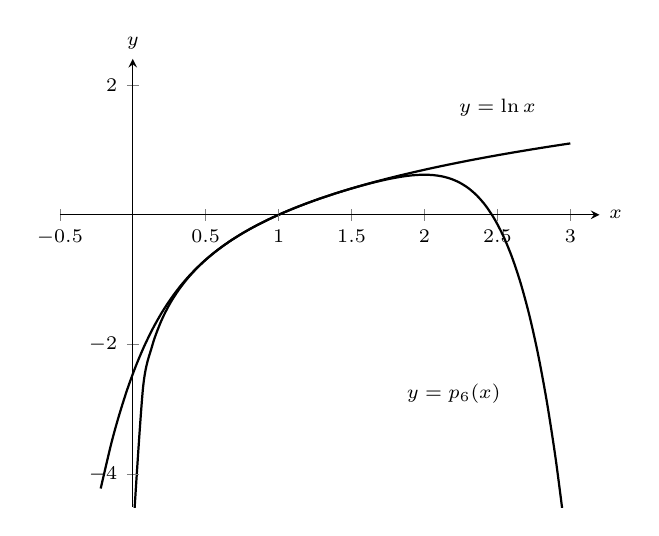
\begin{tikzpicture}
\begin{axis}[ %width=\marginparwidth+25pt,%
tick label style={font=\scriptsize},axis y line=middle,axis x line=middle,name=myplot,axis on top,%
%			xtick={2,4,6,8,10},% 
%			extra x ticks={3.14,1.57},
%			extra x tick labels={$\pi$,$\pi/2$},
%			ytick={-1,-2,1,2},
			%minor y tick num=1,%extra y ticks={-5,-3,...,7},%
%			minor x tick num=4,
			ymin=-4.5,ymax=2.4,%
			xmin=-.5,xmax=3.2%
]

\addplot [{\colorone},domain=0.01:3,smooth,thick,samples=50] {ln(x)};
\addplot [{\colortwo},domain=-4:4,smooth,thick] coordinates {(-0.22,-4.213)(-0.15,-3.543)(-0.1,-3.132)(-0.04,-2.702)(0.02,-2.333)(0.08,-2.015)(0.14,-1.74)(0.2,
-1.502)(0.26,-1.296)(0.32,-1.115)(0.38,-0.9564)(0.44,-0.8161)(0.5,-0.
6911)(0.56,-0.5791)(0.62,-0.4778)(0.68,-0.3856)(0.74,-0.3011)(0.8,-0.
2231)(0.86,-0.1508)(0.92,-0.08338)(0.98,-0.0202)(1.04,0.03922)(1.1,0.
09531)(1.16,0.1484)(1.22,0.1988)(1.28,0.2468)(1.34,0.2926)(1.4,0.3363)
(1.46,0.378)(1.52,0.4177)(1.58,0.4553)(1.64,0.4907)(1.7,0.5233)(1.76,
0.5527)(1.82,0.578)(1.88,0.5982)(1.94,0.6117)(2.,0.6167)(2.06,0.6108)(
2.12,0.5912)(2.18,0.5544)(2.24,0.4961)(2.3,0.4114)(2.36,0.2944)(2.42,
0.1381)(2.48,-0.06544)(2.54,-0.3253)(2.6,-0.6521)(2.66,-1.058)(2.72,-
1.556)(2.78,-2.161)(2.84,-2.892)(2.9,-3.765)(2.96,-4.804)};
%\addplot [{\colortwo!40},domain=-4:4,thick,smooth] {-x^4/2-x^3/6+x^2+x+2};

\draw (axis cs:2.5,1.65) node {\scriptsize $y=\ln x$};
\draw (axis cs:2.2,-2.75) node {\scriptsize $y=p_{6}(x)$};

\end{axis}

\node [right] at (myplot.right of origin) {\scriptsize $x$};
\node [above] at (myplot.above origin) {\scriptsize $y$};

\end{tikzpicture} %
}
\item	
We approximate $\ln 2$ with $ p_6(2)$:
\begin{align*}
p_6(2) &= (2-1)-\frac12(2-1)^2+\frac13(2-1)^3-\frac14(2-1)^4+\cdots \\
			&\cdots +\frac15(2-1)^5-\frac16(2-1)^6\\
			&=	1-\frac12+\frac13-\frac14+\frac15-\frac16 \\
			&= \frac{37}{60}\\ 
			&\approx 0.616667.
\end{align*}
This approximation is not terribly impressive: a hand held calculator shows that $\ln 2 \approx 0.693147.$ The graph in Figure \ref{fig:taypoly2b} shows that $p_6(x)$ provides less accurate approximations of $\ln x$ as $x$ gets close to 0 or 2. 

Surprisingly enough, even the $20^\text{th}$ degree Taylor polynomial fails to approximate $\ln x$ for $x>2$, as shown in Figure \ref{fig:taypoly2c}. We'll soon discuss why this is.
\mfigure{.5}{A plot of $y=\ln x$ and its 20$^\text{th}$ degree Taylor polynomial at $x=1$.}{fig:taypoly2c}{ %
\begin{tikzpicture}
\begin{axis}[ %width=\marginparwidth+25pt,%
tick label style={font=\scriptsize},axis y line=middle,axis x line=middle,name=myplot,axis on top,%
%			xtick={2,4,6,8,10},% 
%			extra x ticks={3.14,1.57},
%			extra x tick labels={$\pi$,$\pi/2$},
%			ytick={-1,-2,1,2},
			%minor y tick num=1,%extra y ticks={-5,-3,...,7},%
%			minor x tick num=4,
			ymin=-4.5,ymax=2.4,%
			xmin=-.5,xmax=3.2%
]

\addplot [{\colorone},domain=0.01:3,smooth,thick,samples=50] {ln(x)};
\addplot [{\colortwo},domain=-4:4,smooth,thick] coordinates {(-0.108,-7.567)(-0.052,-4.958)(0.004,-3.519)(0.06,-2.671)(0.116,-2.13)
(0.172,-1.756)(0.228,-1.478)(0.284,-1.259)(0.34,-1.079)(0.396,-0.9263)
(0.452,-0.7941)(0.508,-0.6773)(0.564,-0.5727)(0.62,-0.478)(0.676,-0.
3916)(0.732,-0.312)(0.788,-0.2383)(0.844,-0.1696)(0.9,-0.1054)(0.956,-
0.045)(1.012,0.01193)(1.068,0.06579)(1.124,0.1169)(1.18,0.1655)(1.236,
0.2119)(1.292,0.2562)(1.348,0.2986)(1.404,0.3393)(1.46,0.3784)(1.516,
0.4161)(1.572,0.4523)(1.628,0.4874)(1.684,0.5212)(1.74,0.5538)(1.796,
0.5853)(1.852,0.6154)(1.908,0.6427)(1.964,0.6635)(2.02,0.6665)(2.076,
0.621)(2.132,0.4476)(2.188,-0.04877)(2.244,-1.326)(2.3,-4.421)};
%\addplot [{\colortwo!40},domain=-4:4,thick,smooth] {-x^4/2-x^3/6+x^2+x+2};

\draw (axis cs:2.5,1.65) node {\scriptsize $y=\ln x$};
\draw (axis cs:1.7,-2.75) node {\scriptsize $y=p_{20}(x)$};

\end{axis}

\node [right] at (myplot.right of origin) {\scriptsize $x$};
\node [above] at (myplot.above origin) {\scriptsize $y$};

\end{tikzpicture} %
}
\end{enumerate}
}
\end{solution}


\subsection{Taylor's Theorem}

%
Taylor polynomials are used to approximate functions $f(x)$ in mainly two situations:
	\begin{enumerate}
	\item		When $f(x)$ is known, but perhaps ``hard'' to compute directly. For instance, we can define $y=\cos x$ as either the ratio of sides of a right triangle (``adjacent over hypotenuse'') or with the unit circle. However, neither of these provides a convenient way of computing $\cos 2$. A Taylor polynomial of sufficiently high degree can provide a reasonable method of computing such values using only operations usually hard--wired into a computer ($+$, $-$, $\times$ and $\div$).
	
	\item		When $f(x)$ is not known, but information about its derivatives is known. This occurs more often than one might think, especially in the study of differential equations.
	\end{enumerate}

{\textbf{Note:} Even though Taylor polynomials \emph{could} be used in calculators and computers to calculate values of trigonometric functions, in practice they generally aren't. Other more efficient and accurate methods have been developed, such as the CORDIC algorithm.}
	
In both situations, a critical piece of information to have is ``How good is my approximation?'' If we use a Taylor polynomial to compute $\cos 2$, how do we know how accurate the approximation is? 

We had the same problem when studying Numerical Integration. Theorem \ref{thm:numerical_error} provided bounds on the error when using, say, Simpson's Rule to approximate a definite integral. These bounds allowed us to determine that, for instance, using $10$ subintervals provided an approximation within $\pm .01$ of the exact value. The following theorem gives similar bounds for Taylor (and hence Maclaurin) polynomials. 

\begin{theorem}{Taylor's Theorem}{taylorthm}
{\begin{enumerate}
\item	Let $f$ be a function whose $n+1^\text{th}$ derivative exists on an interval $I$ and let $c$ be in $I$. Then, for each $x$ in $I$, there exists $z_x$ between $x$ and $c$ such that
$$f(x) = f(c) + \fp(c)(x-c) + \frac{\fpp(c)}{2!}(x-c)^2+ \cdots +\frac{f\,^{(n)}(c)}{n!}(x-c)^n+R_n(x),$$
where $\ds R_n(x) = \frac{f\,^{(n+1)}(z_x)}{(n+1)!}(x-c)^{(n+1)}.$
\index{Taylor Polynomial!Taylor's Theorem}\index{Taylor's Theorem}

\item		$\ds \big|R_n(x)\big| \leq \frac{\max\left|\,f\,^{(n+1)}(z)\right|}{(n+1)!}\big|(x-c)^{(n+1)}\big|$
\end{enumerate}
}
\end{theorem}

\begin{proof}
The proof requires some cleverness to set up, but then the details are
quite elementary. We define a function $F(t)$ as follows:
$$F(t)=\sum_{k=0}^n{f^{(k)}(t)\over k!}\,(x-t)^k + B(x-t)^{n+1}.$$
(Once we have introduced Taylor series, you will notice that here we have replaced $c$ by $t$ in the first $n+1$ terms of the Taylor series, and added a carefully chosen term on the end, with $B$
to be determined.) Note that
we are temporarily keeping $x$ fixed, so the only variable in this
equation is $t$, and we will be interested
only in $t$ between $c$ and $x$. Now substitute $t=c$:
$$F(c)=\sum_{k=0}^n{f^{(k)}(c)\over k!}\,(x-c)^k + B(x-c)^{n+1}.$$
Set this equal to $f(x)$:
$$f(x)=\sum_{k=0}^n{f^{(k)}(c)\over k!}\,(x-c)^k + B(x-c)^{n+1}.$$
Since $x\not=c$, we can solve this for $B$, which is a
``constant''---it depends on $x$ and $c$ but those are temporarily 
fixed.  Now we
have defined a function $F(t)$ with the property that
$F(c)=f(x)$. Also, all terms with a positive power of
$(x-t)$ become zero when we substitute $x$ for $t$, so
$\ds F(x)=f^{(0)}(x)/0!=f(x)$. So $F(c)=F(x)$. 
By Rolle's theorem (\ref{thm:rolle}), we
know that there is a value $z\in(c,x)$ such that $F'(z)=0$. But what is $F'$?
Each term in $F(t)$, except the first term and the extra
term involving $B$, is a product, so to take the derivative we use the
product rule on each of these terms.
\begin{align*}
  F(t)=f(t)&+{f^{(1)}(t)\over 1!}(x-t)^1+{f^{(2)}(t)\over 2!}(x-t)^2+{f^{(3)}(t)\over 3!}(x-t)^3+\cdots	\\
  &+{f^{(n)}(t)\over n!}(x-t)^n+B(x-t)^{n+1}.
\end{align*}
So the derivative is
\begin{align*}
	  F'(t) = f'(t) &+\left({f^{(1)}(t)\over 1!}(x-t)^0(-1)+{f^{(2)}(t)\over 1!}(x-t)^1\right)	\\
  &+\left({f^{(2)}(t)\over 1!}(x-t)^1(-1)+{f^{(3)}(t)\over 2!}(x-t)^2\right)	\\
  &+\left({f^{(3)}(t)\over 2!}(x-t)^2(-1)+{f^{(4)}(t)\over 3!}(x-t)^3\right)+\dots+	\\
  &+\left({f^{(n)}(t)\over (n-1)!}(x-t)^{n-1}(-1)+{f^{(n+1)}(t)\over n!}(x-t)^n\right)	\\
  &+B(n+1)(x-t)^n(-1).
\end{align*}
The second term in each parenthesis cancel with the first term in the next one,
leaving just
$$F'(t) = {f^{(n+1)}(t)\over n!}(x-t)^n+B(n+1)(x-t)^n(-1).$$
At some $z$, $F'(z)=0$ so
\begin{align*}
  0&={f^{(n+1)}(z)\over n!}(x-z)^n+B(n+1)(x-z)^n(-1)	\\
  B(n+1)(x-z)^n&={f^{(n+1)}(z)\over n!}(x-z)^n	\\
  B&={f^{(n+1)}(z)\over (n+1)!}.
\end{align*}
Now we can write 
$$
  F(t)=\sum_{k=0}^n{f^{(k)}(t)\over k!}\,(x-t)^k + 
  {f^{(n+1)}(z)\over (n+1)!}(x-t)^{n+1}.
$$
Recalling that $F(c)=f(x)$ we get
$$
  f(x)=F(c)=\sum_{k=0}^n{f^{(k)}(c)\over k!}\,(x-c)^k + 
  {f^{(n+1)}(z)\over (n+1)!}(x-a)^{n+1},
$$
which by taking $ z_x=z $ is what we wanted to show.
\end{proof}

The first part of Taylor's Theorem states that $f(x) = p_n(x) + R_n(x)$, where $p_n(x)$ is the $n^\text{th}$ order Taylor polynomial and $R_n(x)$ is the remainder, or error, in the Taylor approximation. The second part gives bounds on how big that error can be. If the $(n+1)^\text{th}$ derivative is large, the error may be large; if $x$ is far from $c$, the error may also be large. However, the $(n+1)!$ term in the denominator tends to ensure that the error gets smaller as $n$ increases.

The following example computes error estimates for the approximations of $\ln 1.5$ and $\ln 2$ made in Example \ref{exa:ex_taypoly2}.\\

\begin{example}{Finding error bounds of a Taylor polynomial}{ex_taypoly3}{
Use Theorem \ref{thm:taylorthm} to find error bounds when approximating $\ln 1.5$ and $\ln 2$ with $p_6(x)$, the Taylor polynomial of degree 6 of $f(x)=\ln x$ at $x=1$, as calculated in Example \ref{exa:ex_taypoly2}. }
\end{example}


\begin{solution}
{\begin{enumerate}
\item	We start with the approximation of $\ln 1.5$ with $p_6(1.5)$. The theorem references an open interval $I$ that contains both $x$ and $c$. The smaller the interval we use the better; it will give us a more accurate (and smaller!) approximation of the error. We let $I = (0.9,1.6)$, as this interval contains both $c=1$ and $x=1.5$. 

The theorem references $\max\big|f\,^{(n+1)}(z)\big|$. In our situation, this is asking ``How big can the $7^\text{th}$ derivative of $y=\ln x$ be on the interval $(0.9,1.6)$?'' The seventh derivative is $y = -6!/x^7$. The largest value it attains on $I$ is about 1506. Thus we can bound the error as:
\begin{align*}
\big|R_6(1.5)\big| &\leq \frac{\max\big|f\,^{(7)}(z)\big|}{7!}\big|(1.5-1)^7\big|\\
					&\leq \frac{1506}{5040}\cdot\frac1{2^7}\\
					&\approx 0.0023.
\end{align*}
\noindent%\drawexampleline
We computed $p_6(1.5) = 0.404688$; using a calculator, we find $\ln 1.5 \approx 0.405465$, so the actual error is about $0.000778$, which is less than our bound of $0.0023$. This affirms Taylor's Theorem; the theorem states that our approximation would be within about 2 thousandths of the actual value, whereas the approximation was actually closer.

\item		We again find an interval $I$ that contains both $c=1$ and $x=2$; we choose $I = (0.9,2.1)$. The maximum value of the seventh derivative of $f$ on this interval is again about 1506 (as the largest values come near $x=0.9$). Thus 
\begin{align*}
\big| R_6(2)\big| &\leq \frac{\max\big|f\,^{(7)}(z)\big|}{7!}\big|(2-1)^7\big|\\
					&\leq \frac{1506}{5040}\cdot1^7\\
					&\approx 0.30.
\end{align*}
This bound is not as nearly as good as before. Using the degree 6 Taylor polynomial at $x =1$ will bring us within 0.3 of the correct answer. As $p_6(2)\approx 0.61667$, our error estimate guarantees that the actual value of $\ln 2$ is somewhere between $0.31667$ and $0.91667$. These bounds are not particularly useful.

In reality, our approximation was only off by about 0.07. However, we are approximating ostensibly because we do not know the real answer. In order to be assured that we have a good approximation, we would have to resort to using a polynomial of higher degree.
\end{enumerate}
}
\end{solution}







We practice again. This time, we use Taylor's theorem to find $n$ that guarantees our approximation is within a certain amount.\\


\begin{example}{Finding sufficiently accurate Taylor polynomials}{ex_taypoly4}{
Find $n$ such that the $n^\text{th}$ Taylor polynomial of $f(x)=\cos x$ at $x=0$ approximates $\cos 2$ to within $0.001$ of the actual answer. What is $p_n(2)$?}
\end{example}


\begin{solution}
{Following Taylor's theorem, we need bounds on the size of the derivatives of $f(x)=\cos x$. In the case of this trigonometric function, this is easy. All derivatives of cosine are $\pm \sin x$ or $\pm \cos x$. In all cases, these functions are never greater than 1 in absolute value. We want the error to be less than $0.001$. To find the appropriate $n$, consider the following inequalities:
\begin{align*}
\frac{\max\big|f\,^{(n+1)}(z)\big|}{(n+1)!}\big|(2-0)^{(n+1)}\big| &\leq 0.001 \\
\frac1{(n+1)!}\cdot2^{(n+1)} &\leq 0.001
\end{align*}
We find an $n$ that satisfies this last inequality with trial--and--error. When $n=8$, we have $\ds \frac{2^{8+1}}{(8+1)!} \approx 0.0014$; when $n=9$, we have $\ds \frac{2^{9+1}}{(9+1)!} \approx 0.000282 <0.001$. Thus we want to approximate $\cos 2$ with $p_9(2)$.\\

We now set out to compute $p_9(x)$. We again need a table of the derivatives of $f(x)=\cos x$ evaluated at $x=0$. A table of these values is given in Table \ref{fig:taypoly4a}.
\mTable{.6}{The derivatives of $f(x)=\cos x$ evaluated at $x=0$.}{fig:taypoly4a}{%
\begin{tabular}{lll}
$f(x) = \cos x $&$\Rightarrow $&$f(0) = 1$\\
$\fp(x) = -\sin x $&$\Rightarrow $&$\fp(0) = 0$\\
$\fp'(x) = -\cos x $&$\Rightarrow $&$\fp'(0) = -1$\\
$\fp''(x) = \sin x $&$\Rightarrow $&$\fp''(0) = 0$\\
$f\,^{(4)}(x) = \cos x $&$\Rightarrow $&$f\,^{(4)}(0) = 1$\\
$f\,^{(5)}(x) = -\sin x $&$\Rightarrow $&$f\,^{(5)}(0) = 0$\\
$f\,^{(6)}(x) = -\cos x $&$\Rightarrow $&$f\,^{(6)}(0) = -1$\\
$f\,^{(7)}(x) = \sin x $&$\Rightarrow $&$f\,^{(7)}(0) = 0$\\
$f\,^{(8)}(x) = \cos x $&$\Rightarrow $&$f\,^{(8)}(0) = 1$\\
$f\,^{(9)}(x) = -\sin x $&$\Rightarrow $&$f\,^{(9)}(0) = 0$
\end{tabular}
}
Notice how the derivatives, evaluated at $x=0$, follow a certain pattern. All the odd powers of $x$ in the Taylor polynomial will disappear as their coefficient is 0. While our error bounds state that we need $p_9(x)$, our work shows that this will be the same as $p_8(x)$. 

Since we are forming our polynomial at $x=0$, we are creating a Maclaurin polynomial, and:
\begin{align*}
p_8(x) &= f(0) + \fp(0)x + \frac{\fpp(0)}{2!}x^2 + \frac{\fp''(0)}{3!}x^3 + \cdots +\frac{f\,^{(8)}}{8!}x^8\\
		&=  1-\frac{1}{2!}x^2+\frac{1}{4!}x^4-\frac{1}{6!}x^6+\frac{1}{8!}x^8
\end{align*}

We finally approximate $\cos 2$:
$$\cos 2 \approx p_8(2) = -\frac{131}{315} \approx -0.41587.$$ Our error bound guarantee that this approximation is within $0.001$ of the correct answer. Technology shows us that our approximation is actually within about $0.0003$ of the correct answer.

Figure \ref{fig:taypoly4b} shows a graph of $y=p_8(x)$ and $y=\cos x$. Note how well the two functions agree on about $(-\pi,\pi)$.

\mfigure{1}{A graph of $f(x)= \cos x$ and its degree 8 Maclaurin polynomial.}{fig:taypoly4b}{ %
\begin{tikzpicture}
\begin{axis}[ %width=\marginparwidth+25pt,%
tick label style={font=\scriptsize},axis y line=middle,axis x line=middle,name=myplot,axis on top,%
			xtick={-5,-4,-3,-2,-1,1,2,3,4,5},% 
%			extra x ticks={3.14,1.57},
%			extra x tick labels={$\pi$,$\pi/2$},
%			ytick={-1,-2,1,2},
			%minor y tick num=1,%extra y ticks={-5,-3,...,7},%
%			minor x tick num=4,
			ymin=-1.1,ymax=1.5,%
			xmin=-5.5,xmax=5.5%
]

\addplot [{\colorone},domain=-5:5,smooth,thick,samples=50] {cos(deg(x))};
\addplot [{\colortwo},domain=-4:4,smooth,thick] coordinates {(-5.,2.528)(-4.8,1.6)(-4.6,0.8894)(-4.4,0.343)(-4.2,-0.0768)(-4.,-0.
3968)(-3.8,-0.6355)(-3.6,-0.8052)(-3.4,-0.9146)(-3.2,-0.9695)(-3.,-0.
9748)(-2.8,-0.9345)(-2.6,-0.8532)(-2.4,-0.7357)(-2.2,-0.5878)(-2.,-0.
4159)(-1.8,-0.2271)(-1.6,-0.02917)(-1.4,0.17)(-1.2,0.3624)(-1.,0.5403)
(-0.8,0.6967)(-0.6,0.8253)(-0.4,0.9211)(-0.2,0.9801)(0,1.)(0.2,0.9801)
(0.4,0.9211)(0.6,0.8253)(0.8,0.6967)(1.,0.5403)(1.2,0.3624)(1.4,0.17)(
1.6,-0.02917)(1.8,-0.2271)(2.,-0.4159)(2.2,-0.5878)(2.4,-0.7357)(2.6,-
0.8532)(2.8,-0.9345)(3.,-0.9748)(3.2,-0.9695)(3.4,-0.9146)(3.6,-0.
8052)(3.8,-0.6355)(4.,-0.3968)(4.2,-0.0768)(4.4,0.343)(4.6,0.8894)(4.
8,1.6)(5.,2.528)};
%\addplot [{\colortwo!40},domain=-4:4,thick,smooth] {-x^4/2-x^3/6+x^2+x+2};

\draw (axis cs:-3.,1) node {\scriptsize $y=p_8(x)$};
%\draw (axis cs:-2,-2.75) node {\scriptsize $y=p_{13}(x)$};

\end{axis}

\node [right] at (myplot.right of origin) {\scriptsize $x$};
\node [above] at (myplot.above origin) {\scriptsize $y$};
\node [below] at (myplot.below origin) {\begin{tikzpicture} \draw[thick,{\colorone}] (0,0)--(10pt,0) node [right,black] {\scriptsize $f(x)= \cos x$};\end{tikzpicture}};
\end{tikzpicture} %
}
}
\end{solution}

\begin{example}{}{}
Find a polynomial approximation for $\sin x$ accurate to $\pm 0.005$ for values of $x$ in $[-\pi/2,\pi/2]$. 
\end{example}
\begin{solution}
From Taylor's theorem with $a=0$:
$$
  \sin x= \sum_{n=0}^N{f^{(n)}(a)\over n!}\,x^n + 
  {f^{(N+1)}(z)\over (N+1)!}x^{N+1}.
$$
What can we say about the size of the term
$${f^{(N+1)}(z)\over (N+1)!}x^{N+1}?$$
Every derivative of $\sin x$ is $\pm\sin x$ or $\pm\cos x$, so
$\ds |f^{(N+1)}(z)|\le 1$.

So we need to pick $N$ so that 
$$\left|{x^{N+1}\over (N+1)!}\right|< 0.005.$$
Since we have limited $x$ to $[-\pi/2,\pi/2]$,
$$\left|{x^{N+1}\over (N+1)!}\right|<{2^{N+1}\over (N+1)!}.$$
The quantity on the right decreases with increasing $N$, so all we
need to do is find an $N$ so that 
$${2^{N+1}\over (N+1)!}<0.005.$$
A little trial and error shows that $N=8$ works, 
and in fact $\ds 2^{9}/9!<0.0015$, so 
\begin{align*}
  \sin x &=\sum_{n=0}^8{f^{(n)}(0)\over n!}\,x^n \pm 0.0015	\\
  &=x-{x^3\over 6}+{x^5\over 120}-{x^7\over 5040}\pm 0.0015.
\end{align*}
Figure~\ref{fig:sine approximation} shows the graphs of $\sin x$ and
and the approximation on $[0,3\pi/2]$. As $x$ gets larger, the
approximation heads to negative infinity very quickly, since it is
essentially acting like $\ds -x^7$.
\end{solution}

\begin{figure}[H]
%\texonly
\centerline{
\vbox{\beginpicture
\normalgraphs
%\ninepoint
\setcoordinatesystem units <2truecm,0.7truecm>
\setplotarea x from 0 to 5, y from -5 to 1
\axis left ticks numbered from -5 to 1 by 1 /
\axis bottom shiftedto y=0 ticks numbered from 1 to 5 by 1 /
\setquadratic
\plot 0.000 0.000 0.047 0.047 0.094 0.094 0.141 0.141 0.188 0.187 
0.236 0.233 0.283 0.279 0.330 0.324 0.377 0.368 0.424 0.412 
0.471 0.454 0.518 0.495 0.565 0.536 0.613 0.575 0.660 0.613 
0.707 0.649 0.754 0.685 0.801 0.718 0.848 0.750 0.895 0.780 
0.942 0.809 0.990 0.836 1.037 0.861 1.084 0.884 1.131 0.905 
1.178 0.924 1.225 0.941 1.272 0.956 1.319 0.969 1.367 0.979 
1.414 0.988 1.461 0.994 1.508 0.998 1.555 1.000 1.602 0.999 
1.649 0.997 1.696 0.992 1.744 0.985 1.791 0.975 1.838 0.964 
1.885 0.950 1.932 0.934 1.979 0.917 2.026 0.896 2.073 0.874 
2.121 0.850 2.168 0.824 2.215 0.796 2.262 0.766 2.309 0.735 
2.356 0.701 2.403 0.666 2.450 0.629 2.498 0.591 2.545 0.550 
2.592 0.509 2.639 0.466 2.686 0.421 2.733 0.375 2.780 0.328 
2.827 0.279 2.875 0.230 2.922 0.179 2.969 0.126 3.016 0.073 
3.063 0.018 3.110 -0.037 3.157 -0.094 3.204 -0.152 3.252 -0.212 
3.299 -0.272 3.346 -0.334 3.393 -0.397 3.440 -0.461 3.487 -0.527 
3.534 -0.595 3.581 -0.664 3.629 -0.735 3.676 -0.808 3.723 -0.884 
3.770 -0.962 3.817 -1.042 3.864 -1.125 3.911 -1.212 3.958 -1.302 
4.006 -1.395 4.053 -1.493 4.100 -1.596 4.147 -1.703 4.194 -1.816 
4.241 -1.936 4.288 -2.061 4.335 -2.194 4.383 -2.335 4.430 -2.484 
4.477 -2.642 4.524 -2.811 4.571 -2.990 4.618 -3.181 4.665 -3.385 
4.712 -3.602 /
\plot 0.000 0.000 0.047 0.047 0.094 0.094 0.141 0.141 0.188 0.187 
0.236 0.233 0.283 0.279 0.330 0.324 0.377 0.368 0.424 0.412 
0.471 0.454 0.518 0.495 0.565 0.536 0.613 0.575 0.660 0.613 
0.707 0.649 0.754 0.685 0.801 0.718 0.848 0.750 0.895 0.780 
0.942 0.809 0.990 0.836 1.037 0.861 1.084 0.884 1.131 0.905 
1.178 0.924 1.225 0.941 1.272 0.956 1.319 0.969 1.367 0.979 
1.414 0.988 1.461 0.994 1.508 0.998 1.555 1.000 1.602 1.000 
1.649 0.997 1.696 0.992 1.744 0.985 1.791 0.976 1.838 0.965 
1.885 0.951 1.932 0.935 1.979 0.918 2.026 0.898 2.073 0.876 
2.121 0.853 2.168 0.827 2.215 0.800 2.262 0.771 2.309 0.740 
2.356 0.707 2.403 0.673 2.450 0.637 2.498 0.600 2.545 0.562 
2.592 0.522 2.639 0.482 2.686 0.440 2.733 0.397 2.780 0.353 
2.827 0.309 2.875 0.264 2.922 0.218 2.969 0.172 3.016 0.125 
3.063 0.078 3.110 0.031 3.157 -0.016 3.204 -0.063 3.252 -0.110 
3.299 -0.156 3.346 -0.203 3.393 -0.249 3.440 -0.294 3.487 -0.339 
3.534 -0.383 3.581 -0.426 3.629 -0.468 3.676 -0.509 3.723 -0.549 
3.770 -0.588 3.817 -0.625 3.864 -0.661 3.911 -0.696 3.958 -0.729 
4.006 -0.760 4.053 -0.790 4.100 -0.818 4.147 -0.844 4.194 -0.869 
4.241 -0.891 4.288 -0.911 4.335 -0.930 4.383 -0.946 4.430 -0.960 
4.477 -0.972 4.524 -0.982 4.571 -0.990 4.618 -0.996 4.665 -0.999 
4.712 -1.000 /
\endpicture}}
\caption{$\sin x$ and a polynomial approximation.}
\label{fig:sine approximation}
%\endtexonly
\end{figure}

Note that we can now approximate the value of $\sin(x)$ to within $ 0.005 $ by
using simple trigonometric identities to translate $x$ into the interval $[-\pi/2,\pi/2]$.

\begin{example}{}{}
Find a polynomial approximation for $\ds e^x$ near $x=2$
accurate to $\pm 0.005$. 
\end{example}
\begin{solution}
From Taylor's theorem:
$$
  e^x= \sum_{n=0}^N{e^2\over n!}\,(x-2)^n + 
  {e^z\over (N+1)!}(x-2)^{N+1},
$$
since $\ds f^{(n)}(x)=e^x$ for all $n$. We are interested in $x$ near 2,
and we need to keep $\ds |(x-2)^{N+1}|$ in check, so we may as well
specify that $|x-2|\le 1$, so $x\in[1,3]$. Also
$$\left|{e^z\over (N+1)!}\right|\le {e^3\over (N+1)!},$$
so we need to find an $N$ that makes $\ds e^3/(N+1)!\le 0.005$. This time
$N=5$ makes $\ds e^3/(N+1)!< 0.0015$, so the approximating polynomial is
$$
  e^x=e^2+e^2(x-2)+{e^2\over2}(x-2)^2+{e^2\over6}(x-2)^3+
  {e^2\over24}(x-2)^4+{e^2\over120}(x-2)^5
  \pm 0.0015.
$$

Note that our approximation requires that we already have a very
accurate approximation of the value $e^2$, which we shouldn't assume
we have in the context of trying to approximate $e^x$. For this reason
we typically try to center our series on values for which the derivative
of the function is easy to evaluate (e.g. $a=0$).
\end{solution}

Note well that in these examples we found polynomials of a certain
accuracy only on a small interval, even though the series for $\sin x$
and $\ds e^x$ converge for all $x$; this is typical. To get the same
accuracy on a larger interval would require more terms. 


%

\begin{example}{Finding and using Taylor polynomials}{ex_taypoly5}{
\begin{enumerate}
					\item		Find the degree 4 Taylor polynomial, $p_4(x)$, for $f(x)=\sqrt{x}$ at $x=4.$
					\item		Use $p_4(x)$ to approximate $\sqrt{3}$.
					\item		Find bounds on the error when approximating $\sqrt{3}$ with $p_4(3)$.
					\end{enumerate}
}
\end{example}


\begin{solution}
{\begin{enumerate}
\item		We begin by evaluating the derivatives of $f$ at $x=4$. This is done in Figure \ref{fig:taypoly5a}.
\mTable{.75}{The derivatives of $f(x)=\sqrt{x}$ evaluated at $x=4$.}{fig:taypoly5a}{%
\begin{tabular}{lll}
$f(x) = \sqrt{x} $&$\Rightarrow $&$f(4) = 2$\rule[-12pt]{0pt}{5pt}\\
$\ds\fp(x) = \frac{1}{2\sqrt{x}} $&$\Rightarrow $&$\ds\fp(4) = \frac{1}{4}$\rule[-12pt]{0pt}{5pt}\\
$\ds\fp'(x) = \frac{-1}{4x^{3/2}} $&$\Rightarrow $&$\ds\fp'(4) = \frac{-1}{32}$\rule[-12pt]{0pt}{5pt}\\
$\ds\fp''(x) = \frac3{8x^{5/2}} $&$\Rightarrow $&$\ds\fp''(4) = \frac{3}{256}$\rule[-12pt]{0pt}{5pt}\\
$\ds f\,^{(4)}(x) = \frac{-15}{16x^{7/2}} $&$\Rightarrow $&$\ds f\,^{(4)}(4) = \frac{-15}{2048}$
\end{tabular}
}
These values allow us to form the Taylor polynomial $p_4(x)$:
$$p_4(x) = 2 + \frac14(x-4) +\frac{-1/32}{2!}(x-4)^2+\frac{3/256}{3!}(x-4)^3+\frac{-15/2048}{4!}(x-4)^4.$$

\item		As $p_4(x) \approx \sqrt{x}$ near $x=4$, we approximate $\sqrt{3}$ with $p_4(3) = 1.73212$.
%\enlargethispage{3\baselineskip}

\item		To find a bound on the error, we need an open interval that contains $x=3$ and $x=4$. We set $I = (2.9,4.1)$. The largest value the fifth derivative of $f(x)=\sqrt{x}$ takes on this interval is near $x=2.9$, at about $0.0273$. Thus 
$$\big|R_4(3)\big| \leq \frac{0.0273}{5!}\big|(3-4)^5\big| \approx 0.00023.$$
This shows our approximation is accurate to at least the first 2 places after the decimal. (It turns out that our approximation is actually accurate to 4 places after the decimal.) A graph of $f(x)=\sqrt x$ and $p_4(x)$ is given in Figure \ref{fig:taypoly5b}. Note how the two functions are nearly indistinguishable on $(2,7)$.

\mfigure{1}{A graph of $f(x)=\sqrt{x}$ and its degree 4 Taylor polynomial at $x=4$.}{fig:taypoly5b}{ %
\begin{tikzpicture}
\begin{axis}[ %width=\marginparwidth+25pt,%
tick label style={font=\scriptsize},axis y line=middle,axis x line=middle,name=myplot,axis on top,%
%			xtick={-5,-4,-3,-2,-1,1,2,3,4,5},% 
%			extra x ticks={3.14,1.57},
%			extra x tick labels={$\pi$,$\pi/2$},
%			ytick={-1,-2,1,2},
			%minor y tick num=1,%extra y ticks={-5,-3,...,7},%
%			minor x tick num=4,
			ymin=-.1,ymax=3.5,%
			xmin=-1,xmax=11%
]

\addplot [{\colorone},domain=0:10,smooth,thick,samples=50] coordinates {(0,0)(0.016,0.1265)(0.032,0.1789)(0.048,0.2191)(0.064,0.253)(0.08,0.2828)(0.096,0.3098)(0.112,0.3347)(0.128,0.3578)(0.144,0.3795)(0.16,0.4)(0.176,0.4195)(0.192,0.4382)(0.208,0.4561)(0.224,0.4733)(0.24,0.4899)(0.256,0.506)(0.272,0.5215)(0.288,0.5367)(0.304,0.5514)(0.32,0.5657)(0.336,0.5797)(0.352,0.5933)(0.368,0.6066)(0.384,0.6197)(0.4,0.6325)(0.8,0.8944)(1.2,1.095)(1.6,1.265)(2.,1.414)(2.4,1.549)(2.8,1.673)(3.2,1.789)(3.6,1.897)(4.,2.)(4.4,2.098)(4.8,2.191)(5.2,2.28)(5.6,2.366)(6.,2.449)(6.4,2.53)(6.8,2.608)(7.2,2.683)(7.6,2.757)(8.,2.828)(8.4,2.898)(8.8,2.966)(9.2,3.033)(9.6,3.098)(10.,3.162)};
\addplot [{\colortwo},smooth,thick] coordinates {(0,0.5469)(0.2,0.6536)(0.4,0.7551)(0.6,0.8518)(0.8,0.944)(1.,1.032)(1.
2,1.116)(1.4,1.196)(1.6,1.273)(1.8,1.346)(2.,1.417)(2.2,1.485)(2.4,1.
55)(2.6,1.613)(2.8,1.673)(3.,1.732)(3.2,1.789)(3.4,1.844)(3.6,1.897)(
3.8,1.949)(4.,2.)(4.2,2.049)(4.4,2.098)(4.6,2.145)(4.8,2.191)(5.,2.
236)(5.2,2.28)(5.4,2.324)(5.6,2.366)(5.8,2.408)(6.,2.448)(6.2,2.488)(
6.4,2.527)(6.6,2.565)(6.8,2.602)(7.,2.637)(7.2,2.672)(7.4,2.705)(7.6,
2.737)(7.8,2.768)(8.,2.797)(8.2,2.824)(8.4,2.849)(8.6,2.873)(8.8,2.
894)(9.,2.913)(9.2,2.929)(9.4,2.942)(9.6,2.953)(9.8,2.96)(10.,2.964)};
%\addplot [{\colortwo!40},domain=-4:4,thick,smooth] {-x^4/2-x^3/6+x^2+x+2};

\draw (axis cs:8.,1) node {\begin{tikzpicture}
						\draw[thick,{\colorone}] (0,0)--(10pt,0) node [right,black] {\scriptsize $y= \sqrt x$};
						\draw[{\colortwo},thick] (0,-10pt)--(10pt,-10pt) node [right,black] {\scriptsize $y= p_4(x)$};
													\end{tikzpicture}};
%\draw (axis cs:-2,-2.75) node {\scriptsize $y=p_{13}(x)$};



\end{axis}

\node [right] at (myplot.right of origin) {\scriptsize $x$};
\node [above] at (myplot.above origin) {\scriptsize $y$};
%\node [below] at (myplot.below origin) {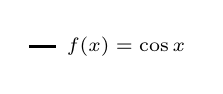
\begin{tikzpicture} \draw[thick,{\colorone}] (0,0)--(10pt,0) node [right,black] {\scriptsize $f(x)= \cos x$};\end{tikzpicture}};

\end{tikzpicture}
}
\end{enumerate}
}
\end{solution}




%\clearpage
%
Our final example gives a brief introduction to using Taylor polynomials to solve differential equations.\\


\begin{example}{Approximating an unknown function}{ex_taypoly6}
{
A function $y=f(x)$ is unknown save for the following two facts.
\begin{enumerate}
\item		$y(0) = f(0) = 1$, and
\item		$y\primeskip'= y^2$
\end{enumerate}
(This second fact says that amazingly, the derivative of the function is actually the function squared!)

Find the degree 3 Maclaurin polynomial $p_3(x)$ of $y=f(x)$.
}
\end{example}


\begin{solution}
{One might initially think that not enough information is given to find $p_3(x)$. However, note how the second fact above actually lets us know what $y\primeskip'(0)$ is:
$$y\primeskip' = y^2 \Rightarrow y\primeskip'(0) = y^2(0).$$
Since $y(0) = 1$, we conclude that $y\primeskip'(0) = 1$.

%\drawexampleline
Now we find information about $y\primeskip''$. Starting with $y\primeskip'=y^2$, take derivatives of both sides, \emph{with respect to $x$}. That means we must use implicit differentiation.
\begin{align*}
y\primeskip' &= y^2\\
\frac{d}{dx}\big(y\primeskip'\big) &= \frac{d}{dx}\big(y^2\big)\\
y\primeskip'' &= 2y\cdot y\primeskip'.
\intertext{Now evaluate both sides at $x=0$:}
y\primeskip''(0) &= 2y(0)\cdot y\primeskip'(0)\\
y\primeskip''(0) &= 2
\end{align*}
We repeat this once more to find $y\primeskip'''(0)$. We again use implicit differentiation; this time the Product Rule is also required.
\begin{align*}
\frac{d}{dx}\big(y\primeskip''\big) &= \frac{d}{dx} \big(2yy\primeskip'\big)\\
y\primeskip''' &= 2y\primeskip'\cdot y\primeskip' + 2y\cdot y\primeskip''.
\intertext{Now evaluate both sides at $x=0$:}
y\primeskip'''(0) &= 2y\primeskip'(0)^2 + 2y(0)y\primeskip''(0)\\
y\primeskip'''(0) &=	2+4=6
\end{align*}
In summary, we have:
$$y(0) = 1 \qquad y\primeskip'(0) = 1  \qquad y\primeskip''(0) = 2 \qquad y\primeskip'''(0) = 6.$$
We can now form $p_3(x)$:
\begin{align*}
p_3(x) &= 1 + x + \frac{2}{2!}x^2 + \frac{6}{3!}x^3\\
				&= 1+x+x^2+x^3.
\end{align*}
\mfigure{.8}{A graph of $y=-1/(x-1)$ and $y=p_3(x)$ from Example \ref{exa:ex_taypoly6}.}{fig:taypoly6}{ %
\begin{tikzpicture}
\begin{axis}[ %width=\marginparwidth+25pt,%
tick label style={font=\scriptsize},axis y line=middle,axis x line=middle,name=myplot,axis on top,%
%			xtick={-5,-4,-3,-2,-1,1,2,3,4,5},% 
%			extra x ticks={3.14,1.57},
%			extra x tick labels={$\pi$,$\pi/2$},
%			ytick={-1,-2,1,2},
			%minor y tick num=1,%extra y ticks={-5,-3,...,7},%
%			minor x tick num=4,
			ymin=-.1,ymax=3.5,%
			xmin=-1.1,xmax=1.1%
]

\addplot [{\colorone},domain=-1:.7,smooth,thick,samples=50] {-1/(x-1)};
\addplot [{\colortwo},smooth,thick] coordinates {(-1.,0)(-0.96,0.07686)(-0.92,0.1477)(-0.88,0.2129)(-0.84,0.2729)(-0.8,
0.328)(-0.76,0.3786)(-0.72,0.4252)(-0.68,0.468)(-0.64,0.5075)(-0.6,0.
544)(-0.56,0.578)(-0.52,0.6098)(-0.48,0.6398)(-0.44,0.6684)(-0.4,0.
696)(-0.36,0.7229)(-0.32,0.7496)(-0.28,0.7764)(-0.24,0.8038)(-0.2,0.
832)(-0.16,0.8615)(-0.12,0.8927)(-0.08,0.9259)(-0.04,0.9615)(0,1.)(0.
04,1.042)(0.08,1.087)(0.12,1.136)(0.16,1.19)(0.2,1.248)(0.24,1.311)(0.
28,1.38)(0.32,1.455)(0.36,1.536)(0.4,1.624)(0.44,1.719)(0.48,1.821)(0.
52,1.931)(0.56,2.049)(0.6,2.176)(0.64,2.312)(0.68,2.457)(0.72,2.612)(
0.76,2.777)(0.8,2.952)(0.84,3.138)(0.88,3.336)(0.92,3.545)(0.96,3.766)(1.,4.)};
%\addplot [{\colortwo!40},domain=-4:4,thick,smooth] {-x^4/2-x^3/6+x^2+x+2};

\draw (axis cs:.75,.9) node {\begin{tikzpicture}
						\draw[thick,{\colorone}] (0,0)--(10pt,0) node [right,black] {\scriptsize $\displaystyle y= \frac{1}{1-x}$};
						\draw[{\colortwo},thick] (0,-15pt)--(10pt,-15pt) node [right,black] {\scriptsize $y= p_3(x)$};
													\end{tikzpicture}};
%\draw (axis cs:-2,-2.75) node {\scriptsize $y=p_{13}(x)$};



\end{axis}

\node [right] at (myplot.right of origin) {\scriptsize $x$};
\node [above] at (myplot.above origin) {\scriptsize $y$};
%\node [below] at (myplot.below origin) {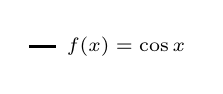
\begin{tikzpicture} \draw[thick,{\colorone}] (0,0)--(10pt,0) node [right,black] {\scriptsize $f(x)= \cos x$};\end{tikzpicture}};

\end{tikzpicture} %
}
It turns out that the differential equation we started with, $y\primeskip'=y^2$, where $y(0)=1$, can be solved without too much difficulty: $\ds y = \frac{1}{1-x}$. Figure \ref{fig:taypoly6} shows this function plotted with $p_3(x)$. Note how similar they are near $x=0$.
} 
\end{solution}


It is beyond the scope of this text to pursue error analysis when using Taylor polynomials to approximate solutions to differential equations. This topic is often broached in introductory Differential Equations courses and usually covered in depth in Numerical Analysis courses. Such an analysis is very important; one needs to know how good their approximation is. We explored this example simply to demonstrate the usefulness of Taylor polynomials. \\

Most of this chapter has been devoted to the study of infinite series. This section has taken a step back from this study, focusing instead on finite summation of terms. In the next section, we explore {\textit{Taylor Series}}, where we represent a function with an infinite series.

%%%%%%%%%%%%%%%%%%%%%%%%%%%%%%%%%%%%%%%%%%%%
\Opensolutionfile{solutions}[ex]
\section*{Exercises for \ref{sec:taylorpolynomials}}

\begin{enumialphparenastyle}

% % % % % % % % % % %
\begin{ex}
Find the Maclaurin polynomial of degree $n$ for the given function.
\begin{enumerate}
\item {$f(x) = e^{-x}, \quad n=3$
}
\item {$f(x) = \sin x, \quad n=8$
}
\item {$f(x) = x\cdot e^x, \quad n=5$
}
\item {$f(x) = \tan x, \quad n=6$
}
\item {$f(x) = e^{2x}, \quad n=4$
}
\item {$\ds f(x) = \frac1{1-x}, \quad n=4$
}
\item {$\ds f(x) = \frac1{1+x}, \quad n=4$
}
\item {$\ds f(x) = \frac1{1+x}, \quad n=7$
}
\end{enumerate}

\begin{sol}
\begin{enumerate}
\item 
{$p_3(x) = 1-x+\frac12x^3-\frac16x^3$
}
\item 
{$p_8(x) = x-\frac16x^3+\frac1{120}x^5-\frac1{5040}x^7$
}
\item 
{$p_8(x) = x+x^2+\frac12x^3+\frac16x^4+\frac1{24}x^5$
}
\item 
{$p_6(x) = \frac{2 x^5}{15}+\frac{x^3}{3}+x$
}
\item 
{$p_4(x) = \frac{2 x^4}{3}+\frac{4 x^3}{3}+2 x^2+2 x+1$
}
\item 
{$p_4(x) = x^4+x^3+x^2+x+1$
}
\item 
{$p_4(x) = x^4-x^3+x^2-x+1$
}
\item 
{$p_7(x) = -\frac{x^7}{7}+\frac{x^5}{5}-\frac{x^3}{3}+x$
}
\end{enumerate}
\end{sol}

\end{ex}
% % % % % % % % % % % %

% % % % % % % % % % %
\begin{ex}
Find the Taylor polynomial of degree $n$, at $x=c$, for the given function.
\begin{enumerate}
\item {$\ds f(x) = \sqrt x, \quad n=4, \quad c=1$
}
\item {$\ds f(x) = \ln (x+1), \quad n=4, \quad c=1$
}
\item {$\ds f(x) = \cos x, \quad n=6, \quad c=\pi/4$
}
\item {$\ds f(x) = \sin x, \quad n=5, \quad c=\pi/6$
}
\item {$\ds f(x) = \frac1x, \quad n=5, \quad c=2$
}
\item  {$\ds f(x) = \frac{1}{x^2}, \quad n=8, \quad c=1$
}
\item {$\ds f(x) = \frac{1}{x^2+1}, \quad n=3, \quad c=-1$
}
\item {$\ds f(x) = x^2\cos x, \quad n=2, \quad c=\pi$
}
\end{enumerate}

\begin{sol}
\begin{enumerate}
\item 
{$p_4(x) = 1+\frac{1}{2} (-1+x)-\frac{1}{8} (-1+x)^2+\frac{1}{16}
   (-1+x)^3-\frac{5}{128} (-1+x)^4$
}
\item 
{$p_4(x) = \ln (2)+\frac{1}{2} (-1+x)-\frac{1}{8}
   (-1+x)^2+\frac{1}{24} (-1+x)^3-\frac{1}{64} (-1+x)^4$
}
\item 
{$p_6(x) = \frac{1}{\sqrt{2}}-\frac{-\frac{\pi
   }{4}+x}{\sqrt{2}}-\frac{\left(-\frac{\pi
   }{4}+x\right)^2}{2 \sqrt{2}}+\frac{\left(-\frac{\pi
   }{4}+x\right)^3}{6 \sqrt{2}}+\frac{\left(-\frac{\pi
   }{4}+x\right)^4}{24 \sqrt{2}}-\frac{\left(-\frac{\pi
   }{4}+x\right)^5}{120 \sqrt{2}}-\frac{\left(-\frac{\pi
   }{4}+x\right)^6}{720 \sqrt{2}}$
}
\item 
{$p_5(x) = \frac{1}{2}+\frac{1}{2} \sqrt{3} \left(-\frac{\pi
   }{6}+x\right)-\frac{1}{4} \left(-\frac{\pi
   }{6}+x\right)^2-\frac{\left(-\frac{\pi }{6}+x\right)^3}{4
   \sqrt{3}}+\frac{1}{48} \left(-\frac{\pi
   }{6}+x\right)^4+\frac{\left(-\frac{\pi
   }{6}+x\right)^5}{80 \sqrt{3}}$
}
\item 
{$p_5(x) = \frac{1}{2}-\frac{x-2}{4}+\frac{1}{8} (x-2)^2-\frac{1}{16}
   (x-2)^3+\frac{1}{32} (x-2)^4-\frac{1}{64} (x-2)^5$
}
\item
{$p_8(x) = 1-2 (-1+x)+3 (-1+x)^2-4 (-1+x)^3+5 (-1+x)^4-6 (-1+x)^5+7
   (-1+x)^6-8 (-1+x)^7+9 (-1+x)^8$
}
\item 
{$p_3(x) =\frac{1}{2}+\frac{1+x}{2}+\frac{1}{4} (1+x)^2$
}
\item 
{$p_2(x) =-\pi ^2-2 \pi  (x-\pi)+\frac{1}{2} \left(\pi ^2-2\right)
   (x-\pi)^2$
}
\end{enumerate}
\end{sol}

\end{ex}
% % % % % % % % % % % %

% % % % % % % % % % %
\begin{ex}
Approximate the function value with the indicated Taylor polynomial and give approximate bounds on the error.
\begin{enumerate}
\item {Approximate $\sin 0.1$ with the Maclaurin polynomial of degree 3.
}
\item {Approximate $\cos 1$ with the Maclaurin polynomial of degree 4.
}
\item {Approximate $\sqrt{10}$ with the Taylor polynomial of degree 2 centered at $x=9$.
}
\item {Approximate $\ln1.5$ with the Taylor polynomial of degree 3 centered at $x=1$.
}
\end{enumerate}

\begin{sol}
\begin{enumerate}
\item 
{$p_3(x) =x-\frac{x^3}{6}$; $p_3(0.1) = 0.09983$. Error is bounded by $\pm \frac{1}{4!}\cdot0.1^4 \approx \pm 0.000004167$.
}
\item 
{$p_4(x) =1-\frac{x^2}{2}+\frac{x^4}{24}$; $p_4(1) = 13/24\approx 0.54167$. Error is bounded by $\pm \frac{1}{5!}\cdot1^5 \approx \pm 0.00833$
}
\item 
{$p_2(x) =3+\frac{1}{6} (-9+x)-\frac{1}{216} (-9+x)^2$; $p_2(10) =  3.16204$. The third derivative of $f(x) =\sqrt x$ is bounded on $(8,11)$ by $0.003$. Error is bounded by $\pm \frac{0.003}{3!}\cdot1^3 = \pm 0.0005.$
}
\item 
{$p_3(x) =-1+x-\frac{1}{2} (-1+x)^2+\frac{1}{3} (-1+x)^3$; $p_3(1.5) =  0.41667$. The fourth derivative of $f(x) =\ln x$ is bounded on $(.9,2)$ by $10$. Error is bounded by $\pm \frac{10}{4!}\cdot.5^4 = \pm 0.026.$
}
\end{enumerate}
\end{sol}

\end{ex}
% % % % % % % % % % % %

% % % % % % % % % % %
\begin{ex}
Find an $n$  such that $p_n(x)$ approximates $f(x)$ within the specified bound of accuracy.
\begin{enumerate}
\item {Find $n$ such that the  Maclaurin polynomial of degree $n$ of $f(x)= e^x$ approximates $e$ within $0.0001$ of the actual value.
}
\item {Find $n$ such that the  Taylor polynomial of degree $n$ of $f(x)= \sqrt x$, centered at $x=4$, approximates $\sqrt 3$ within $0.0001$ of the actual value.
}
\item {Find $n$ such that the  Maclaurin polynomial of degree $n$ of $f(x)= \cos x$ approximates $\cos \pi/3$ within $0.0001$ of the actual value.
}
\item {Find $n$ such that the  Maclaurin polynomial of degree $n$ of $f(x)= \sin x$ approximates $\cos \pi$ within $0.0001$ of the actual value.
}
\end{enumerate}

\begin{sol}
\begin{enumerate}
\item 
{The $n^\text{th}$ derivative of $f(x)=e^x$ is bounded by $3$ on intervals containing $0$ and 1. Thus $|R_n(1)|\leq \frac{3}{(n+1)!}1^{(n+1)}$. When $n=7$, this is less than $0.0001$. 
}
\item 
{The $n^\text{th}$ derivative of $f(x)=\sqrt x$ is bounded by $0.1$ on intervals containing $3$ and $4$. Thus $|R_n(\pi)|\leq \frac{0.1}{(n+1)!}(1)^{(n+1)}$. When $n=4$, this is less than $0.0001$.
}
\item 
{The $n^\text{th}$ derivative of $f(x)=\cos x$ is bounded by $1$ on intervals containing $0$ and $\pi/3$. Thus $|R_n(\pi/3)|\leq \frac{1}{(n+1)!}(\pi/3)^{(n+1)}$. When $n=7$, this is less than $0.0001$. Since the Maclaurin polynomial of $\cos x$ only uses even powers, we can actually just use $n=6$.
}
\item 
{The $n^\text{th}$ derivative of $f(x)=\sin x$ is bounded by $1$ on intervals containing $0$ and $\pi$. Thus $|R_n(\pi)|\leq \frac{1}{(n+1)!}(\pi)^{(n+1)}$. When $n=12$, this is less than $0.0001$. Since the Maclaurin polynomial of $\sin x$ only uses odd powers, we can actually just use $n=11$.
}
\end{enumerate}
\end{sol}

\end{ex}
% % % % % % % % % % % %

% % % % % % % % % % %
\begin{ex}
Find the $n^\text{th}$ term of the indicated Taylor polynomial.
\begin{enumerate}
\item {Find a formula for the $n^\text{th}$ term of the Maclaurin polynomial for $f(x)=e^x$.
}
\item {Find a formula for the $n^\text{th}$ term of the Maclaurin polynomial for $f(x)=\cos x$.
}
\item {Find a formula for the $n^\text{th}$ term of the Maclaurin polynomial for $\ds f(x)=\frac{1}{1-x}$.
}
\item {Find a formula for the $n^\text{th}$ term of the Maclaurin polynomial for $\ds f(x)=\frac{1}{1+x}$.
}
\item {Find a formula for the $n^\text{th}$ term of the Taylor polynomial for $\ds f(x)=\ln x$.
}
\end{enumerate}

\begin{sol}
\begin{enumerate}
\item 
{The $n^\text{th}$ term is $\frac{1}{n!}x^n$.
}
\item 
{The $n^\text{th}$ term is: when $n$ is even,  $\frac{(-1)^{n/2}}{n!}x^n$; when $n$ is odd, $0$.
}
\item 
{The $n^\text{th}$ term is $x^n$.
}
\item 
{The $n^\text{th}$ term is $(-1)^nx^n$.
}
\item  
{The $n^\text{th}$ term is $(-1)^n\frac{(x-1)^n}{n}$.
}
\end{enumerate}
\end{sol}

\end{ex}
% % % % % % % % % % % %

% % % % % % % % % % %
\begin{ex}
Approximate the solution to the given differential equation with a degree $ 4 $ Maclaurin polynomial.
\begin{enumerate}
\item {$y'=y$, \qquad $y(0) = 1$
}
\item {$y'=5y$,\qquad $y(0) = 3$
}
\item {$\ds y'=\frac2y$,\qquad $y(0) = 1$
}

\end{enumerate}

\begin{sol}
\begin{enumerate}
\item 
{$\ds 1+x+\frac12x^2+\frac16x^3+\frac1{24}x^4$
}
\item 
{$\ds 3+15x+\frac{75}{2}x^2+\frac{375}{6}x^3+\frac{1875}{24}x^4$
}
\item 
{$\ds 1+2x-2x^2+4x^3-10x^4$
}

\end{enumerate}
\end{sol}

\end{ex}

\end{enumialphparenastyle}
% % % % % % % % % % % %


% % % % % % % % % % % %


